\subsection{SD-Karte}\label{sec:sdKarte}

Nachdem nun die ganze Datenübertragung und Kommunikationsebene erklärt wurde, muss jetzt noch die Datenspeicherung und der Datenzugriff verdeutlicht werden. Damit ein Zugriff auf die SD-Karte möglich ist, wurde die Library fatfs verwendet. Sie ermöglicht einen einfachen Zugriff auf die Daten mit einer SPI-Schnittstelle und wird im ersten Kapitel beschrieben. Anschliessend wird die Bündelung des Codes (Modul) in Zusammenhang mit der SD-Karte erklärt. Das letzte Kapitel beschreibt noch die benötigten Files auf der SD-Karte, um die Funktionen des Dōjōs zu gewährleisten.

\subsubsection{FatFs}

Für den Zugriff auf die SD-Karte wird ein Generic FAT Filesystem Module verwendet. In dieser Library sind die Funktionen für die Initialisierung und für den Zugriff auf die SD-Karte enthalten. Die FatFs Library untersteht einer 1-clause BSD Lizenz. Sie darf verwendet werden, muss aber in jedem Fall den Lizenztext beinhalten. Der Lizenztext ist im Kapitel \ref{sec:lizenzen} in der Abbildung \ref{fig:Lizentext FatFs} ersichtlich.

\paragraph{Spezifikationen FatFs}$~~$\\
Dateisystem Typ: FAT, FAT32(rev0.0) und exFAT(rev1.0)\\
Anzahl geöffneter Dateien: unlimitiert (hängt vom verfügbaren Speicher ab)\\
Anzahl Datenträger: bis zu 10\\
Datenträgergrösse: bis zu 2TB bei 512Bytes/Sektor\\
Dateigrösse: bis zu 4GB – 1 auf FAT-Volume und praktisch unbegrenzt auf exFAT-Volume\\
Clustergrösse: Bis zu 128 Sektoren auf FAT-Volume und bis zu 16 MB auf exFAT-Volume	\\
Sektorgrösse:  512, 1024, 2048 und 4096 Bytes \cite{FatFs}\\ 

\subsubsection{SD-Karte Modul}
Das SD-Karten-Modul besteht hauptsächlich aus den Funktionen Merken und SD-Karten-Initialisierung. \textbf{Merken} beinhaltet zwei Funktionen. Die Erste speichert das aktuelle Kunstwerk auf eine Liste, auf welcher die verschieden gemerkten Kunstwerken gesammelt werden. Die zweite Funktion löscht die Liste wieder, um den Dōjō für den nächsten Nutzer betriebsbereit zu machen. Der Dateiname der Liste lässt sich im Header-File konfigurieren. \textbf{SD-Karte Initialisieren} ruft eine Reihe fatfs-Befehle auf, um die SD-Karte zu mounten. Diese wird über einen SPI-Bus an den Mikrocontroller angeschlossen. Die Pins für den Bus lassen sich im Header-File definieren.

\subsubsection{Lookup}
Diese Funktion ist die eigentliche Implementierung des in Abbildung \ref{fig:lookupState} beschrieben Algorithmus und hat mit next\_Value und Sprachwechsel 2 wichtige Funktionen, die nachfolgend beschrieben werden.

\textbf{next\_Value} dient dazu, die nächsten Werte in den Buffer zu laden. Sie ist folgendermassen definiert:
\begin{itemize}
	\item [] \textcolor{red}{static void} next\_value(\textcolor{red}{int} bufix)
\end{itemize}
Sie öffnet zuerst die entsprechende Audiodatei. Dies geschieht nur zu Beginn der Datei. Sie bleibt geöffnet bis die Audiodatei zu Ende ist, oder der Benutzer das Abspielen unterbricht. Ebenfalls wird der Lesezeiger beim ersten Aufruf der Funktion auf das $44$ Byte geschoben, da die ersten $44$ Bytes eines WAV-Files keine Audiodaten enthalten. Die Funktion liest nun 4096 Bytes in einen Hilfsbuffer ein. Die Werte werden dann daraus skaliert und in die Sequenzen geladen. Um eine invertierte Sequenz zu erzeugen, wird das Bit $15$ auf 1 gesetzt.


Die Funktion \textbf{Sprachwechsel} ist für Sprachwechsel des Dōjōs verantwortlich. Die Sprachauswahl geschieht über verschiedene Files. Es exisitert für jede Sprache ein eigenes Lookup-File. Dieses verbindet die Majo-Minor-Kennzeichnungen mit den Wav-Files der jeweiligen Sprache. Dadurch muss für einen Sprachwechsel nur der Zeiger auf das Lookup-File geändert werden.

\subsubsection{Benötigte Files}
Im Header-File des Moduls SD-Karte müssen verschiedene Files definiert werden. Sie müssen auch auf der SD-Karte im richtigen Format vorhanden sein. Die Merken-Liste ist eine normale Textdatei (Endung .txt). Sie sollte leer sein. Des weiteren müssen die Lookup-Files als CSV (Comma separated Value) Dateien vorhanden sein. Sie sollten dem in Abbildung \ref{fig:definition_lookup_file} definierten Format entsprechen. Zu beachten ist, dass die X Symbole für zwei stellige Hex-Zahlen stehen. Somit hat es eine Referenz auf ein Kunstwerk pro Zeile. Weiter gilt, dass die Sprachkürzel nur zwei Zeichen beinhalten sollten.

\begin{figure}[H]
	\begin{center}
		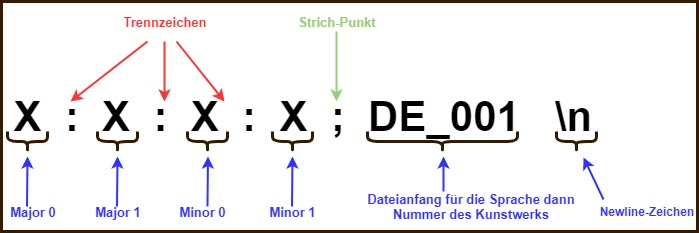
\includegraphics[width=140mm]{data/Definition_file.jpg}
		\caption[Formatdefinition Lookup-File]{Formatdefinition Lookup-File} %picture caption
		\label{fig:definition_lookup_file}
	\end{center}
\end{figure}

Die Audiodateien sind im Format WAV Unsigned 8-bit PCM auf der SD-Karte abzulegen. Dabei muss beachtet werden, dass die Sample Frequenz $32 kHz$ beträgt und es sich um eine Mono-Kanal Datei handelt.
